\documentclass[11pt]{article}
\usepackage{amsmath, amssymb, mathtools, bm}
\usepackage{physics}
\usepackage{tikz}
\usepackage[margin=2.3cm]{geometry}
\usepackage{siunitx, booktabs, hyperref}

\newcommand{\D}{\mathrm{D}}
\newcommand{\de}{\mathrm{d}}
\newcommand{\pd}[2]{\frac{\partial #1}{\partial #2}}
\newcommand{\pdd}[2]{\frac{\partial^{2} #1}{\partial #2^{2}}}
\newcommand{\Lap}{\nabla^{2}}

\title{B1 Fluids --- Trinity Term 2023 \\ Model Solutions}
\author{}
\date{}

\begin{document}
\maketitle

\section*{Question 1 --- Bernoulli, hydrostatics and the sluice gate}

\textbf{Problem statement.} Starting from steady Euler in uniform gravity, derive Bernoulli's theorem along a streamline and interpret it. A reservoir of water of depth $H$ and cross-sectional width $L$ is dammed by a closed sluice gate at $x=0$; show the force on the closed gate is $\rho g H^{2}L/2$. The gate is then raised slightly so that water of speed $U$ and depth $H$ for $x\ll 0$ flows under it and emerges with speed $u$ and depth $h$ for $x\gg 0$. Show that $\hat h = h/H$ satisfies $\hat h = 1$ or $\hat h = (F^{2}+F\sqrt{F^{2}+8})/4$ with $F = U/\sqrt{gH}$, and finally, by writing the momentum budget between far-upstream and far-downstream sections, show that the force on the (raised) gate is $\dfrac{\rho g H^{2} L}{2}\dfrac{(1-\hat h)^{3}}{1+\hat h}$.

\subsection*{(a) Bernoulli's theorem along a streamline}

For a fluid of uniform density $\rho$ in a uniform gravitational field $-g\hat{\bm z}$, the steady inviscid Euler equation reads
\begin{equation}
(\bm v\cdot\nabla)\bm v = -\frac{1}{\rho}\nabla p - g\hat{\bm z}.
\label{eq:euler-steady}
\end{equation}
Each term on the right is a force per unit mass acting on a fluid element; the left-hand side is the convective acceleration of the element along its streamline. The trick is to rewrite the convective term using the vector identity
\begin{equation}
(\bm v\cdot\nabla)\bm v = \nabla\!\left(\tfrac{1}{2}\bm v\cdot\bm v\right) - \bm v\times(\nabla\times\bm v),
\label{eq:vec-id}
\end{equation}
which follows from the standard identity $\nabla(\bm a\cdot\bm a) = 2(\bm a\cdot\nabla)\bm a + 2\bm a\times(\nabla\times\bm a)$. The advantage of \eqref{eq:vec-id} is that it splits the convective term into a pure gradient (the kinetic-energy gradient along the flow) and a part orthogonal to $\bm v$ (the Lamb vector $-\bm v\times\bm\omega$).

Substituting \eqref{eq:vec-id} into \eqref{eq:euler-steady} and noting that $g\hat{\bm z} = \nabla(gz)$ is also a pure gradient, we obtain
\begin{equation}
\nabla\!\left(\frac{\bm v\cdot\bm v}{2} + \frac{p}{\rho} + gz\right) = \bm v\times(\nabla\times\bm v).
\label{eq:bernoulli-grad}
\end{equation}
The right-hand side is by construction perpendicular to $\bm v$. Taking the dot product of \eqref{eq:bernoulli-grad} with $\bm v$ kills the right-hand side, so that the directional derivative of the bracketed quantity along the streamline vanishes:
\begin{equation}
\bm v\cdot\nabla\!\left(\frac{\bm v\cdot\bm v}{2} + \frac{p}{\rho} + gz\right) = 0.
\label{eq:bernoulli-along-s}
\end{equation}
Hence, along any streamline of a steady, inviscid, constant-density flow,
\begin{equation}
\boxed{\;\frac{\bm v\cdot\bm v}{2} + \frac{p}{\rho} + gz = \text{const.}\;}
\label{eq:bernoulli}
\end{equation}

Physically, \eqref{eq:bernoulli} is energy conservation per unit mass for a fluid parcel travelling along a streamline: the three terms are kinetic energy per unit mass, the work done per unit mass by the pressure (the ``flow work''), and the gravitational potential energy per unit mass. As a parcel speeds up along its streamline, either its pressure or its height must drop in compensation; for a horizontal flow this is the familiar Venturi result $p + \tfrac{1}{2}\rho v^{2} = \text{const}$.

\subsection*{(b) Hydrostatic force on a closed sluice gate}

When the gate is closed, the water in $x<0$ is at rest, so $\bm v = 0$ everywhere. Setting $\bm v=0$ in \eqref{eq:euler-steady} (or equivalently in \eqref{eq:bernoulli}) gives the hydrostatic balance
\begin{equation}
\frac{1}{\rho}\nabla p = -g\hat{\bm z} \quad\Longrightarrow\quad p(z) = p_{\text{atm}} + \rho g(H - z),
\label{eq:hydrostatic}
\end{equation}
where we measured $z$ upwards from the bed and used $p = p_{\text{atm}}$ at the free surface $z=H$.

The pressure on the gauge side of the gate is just atmospheric pressure $p_{\text{atm}}$. The net horizontal force on the gate is therefore the integral of the gauge pressure $p - p_{\text{atm}} = \rho g(H-z)$ over the wetted area,
\begin{equation}
F_{\text{gate}} = L\int_{0}^{H}\rho g (H-z)\,\de z = L\,\rho g\!\left[(H-z)\!\left(-\tfrac{(H-z)}{2}\right)\right]_{0}^{H} = \frac{\rho g H^{2}L}{2}.
\label{eq:F-closed}
\end{equation}

\[
\boxed{\;F_{\text{closed}} = \frac{\rho g H^{2} L}{2}.\;}
\]
This is the standard hydrostatic result that the resultant force on a vertical wall holding back a column of fluid equals the pressure at the centroid ($\rho g H/2$) times the wetted area ($H L$).

\subsection*{(c) Two roots of the depth ratio with the gate raised}

When the gate is raised the flow is steady but no longer at rest. Pick a streamline running just under the free surface, from a point far upstream at $x\ll 0$ where the depth is $H$, the speed is $U$ and the pressure is atmospheric, to a point at the downstream free surface at $x\gg 0$ where the depth is $h$, the speed is $u$ and the pressure is again atmospheric. Bernoulli \eqref{eq:bernoulli} on this surface streamline gives, with $z=H$ upstream and $z=h$ downstream,
\begin{equation}
\frac{U^{2}}{2} + \frac{p_{\text{atm}}}{\rho} + gH = \frac{u^{2}}{2} + \frac{p_{\text{atm}}}{\rho} + gh
\;\Longrightarrow\;
\frac{U^{2}}{2} + gH = \frac{u^{2}}{2} + gh.
\label{eq:bern-surface}
\end{equation}

The additional constraint is mass conservation. Because both up- and down-stream profiles are uniform with depth, the volume flux per unit width is the same on each side,
\begin{equation}
U H = u h.
\label{eq:mass}
\end{equation}
This expresses the fact that no water is created or destroyed under the gate; in steady state, what comes in must go out.

Eliminating $u = UH/h$ from \eqref{eq:bern-surface} we obtain
\begin{equation}
\frac{U^{2}}{2} + gH = \frac{U^{2}H^{2}}{2 h^{2}} + gh.
\label{eq:bern-elim}
\end{equation}
Non-dimensionalising with $\hat h = h/H$ and $F^{2} = U^{2}/(gH)$ (the squared upstream Froude number), divide \eqref{eq:bern-elim} by $gH$ to find
\begin{equation}
\frac{F^{2}}{2} + 1 = \frac{F^{2}}{2\hat h^{2}} + \hat h.
\label{eq:bern-nd}
\end{equation}
Multiply through by $2\hat h^{2}$ and rearrange:
\begin{equation}
2\hat h^{3} - (F^{2}+2)\hat h^{2} + F^{2} = 0.
\label{eq:cubic}
\end{equation}
The trivial solution is $\hat h = 1$ (no change in depth, $u=U$, the gate has no effect), which can be checked by substitution; this corresponds to the gate being raised completely out of the water. Factorising $(\hat h - 1)$ out of the cubic in \eqref{eq:cubic},
\begin{equation}
2\hat h^{3} - (F^{2}+2)\hat h^{2} + F^{2} = (\hat h - 1)\!\left[2\hat h^{2} - F^{2}\hat h - F^{2}\right] = 0,
\label{eq:cubic-factored}
\end{equation}
so the non-trivial roots solve the quadratic
\begin{equation}
2\hat h^{2} - F^{2}\hat h - F^{2} = 0.
\label{eq:quadratic}
\end{equation}
Applying the quadratic formula, with discriminant $\Delta = F^{4}+8F^{2} = F^{2}(F^{2}+8)$,
\begin{equation}
\hat h = \frac{F^{2}\pm\sqrt{F^{2}(F^{2}+8)}}{4} = \frac{F^{2}\pm F\sqrt{F^{2}+8}}{4}.
\label{eq:quad-roots}
\end{equation}
The negative root is unphysical (it gives $\hat h < 0$), so we take the positive sign:
\begin{equation}
\boxed{\;\hat h = 1 \quad\text{or}\quad \hat h = \frac{F^{2} + F\sqrt{F^{2}+8}}{4}.\;}
\label{eq:hhat}
\end{equation}
For subcritical upstream flow ($F<1$) one finds $\hat h < 1$, i.e.\ the flow accelerates and thins as it passes under the partially open gate, which is the physically relevant case for a sluice. (The case $\hat h>1$, attained for $F>1$, would correspond to a hydraulic jump under the gate, which is the time-reverse of the present situation and not what the figure shows.)

\subsection*{(d) Momentum budget and the force on the raised gate}

To find the force on the gate we now apply momentum conservation in integral form to the control volume bounded above by the free surface, below by the bed, and on the two ends by vertical sections at $x = -X$ and $x = +X$ with $X$ large enough that the flow there is uniform with depth $H$, $h$ respectively. Steady incompressible momentum conservation applied to this volume reads
\begin{equation}
\dot M_{\text{out}} - \dot M_{\text{in}} = \sum F_{x}^{\text{ext}},
\label{eq:mom-bal}
\end{equation}
where $\dot M_{\text{in}} = \rho U^{2}\!\cdot HL$ is the momentum-flux of water through the upstream face (mass flux $\rho U H L$ times velocity $U$) and $\dot M_{\text{out}} = \rho u^{2}\,hL$ similarly downstream. Using mass conservation \eqref{eq:mass}, $\rho u^{2}h = \rho U^{2}H^{2}/h$, so
\begin{equation}
\dot M_{\text{out}} - \dot M_{\text{in}} = \rho U^{2}H L\!\left(\frac{H}{h}-1\right) = \frac{\rho U^{2} HL\,(1-\hat h)}{\hat h}.
\label{eq:dM}
\end{equation}

The horizontal forces on the control volume are: (i) the hydrostatic pressure force on the upstream face, $+\tfrac{1}{2}\rho g H^{2}L$, pushing right; (ii) the hydrostatic pressure force on the downstream face, $-\tfrac{1}{2}\rho g h^{2}L$, pushing left; and (iii) the reaction force $-F_{\text{gate}}$ exerted by the gate on the fluid (by Newton's third law, equal and opposite to the force we want). The bed is horizontal so contributes no horizontal force, and atmospheric pressure on the free surface contributes nothing horizontal. The hydrostatic profiles are valid at the end sections because the streamlines are straight and horizontal there, so the vertical Euler equation reduces to $\partial_{z} p = -\rho g$ (this is the standard ``shallow-flow'' justification for hydrostatic pressure away from regions of strong vertical curvature).

Combining \eqref{eq:mom-bal}--\eqref{eq:dM},
\begin{equation}
\frac{\rho U^{2} HL\,(1-\hat h)}{\hat h} = \frac{\rho g L}{2}\!\left(H^{2}-h^{2}\right) - F_{\text{gate}}.
\label{eq:mom-explicit}
\end{equation}
Solving for $F_{\text{gate}}$ and using $h = \hat h H$ so that $H^{2}-h^{2} = H^{2}(1-\hat h^{2}) = H^{2}(1-\hat h)(1+\hat h)$,
\begin{equation}
F_{\text{gate}} = \frac{\rho g H^{2} L}{2}(1-\hat h)(1+\hat h) - \frac{\rho U^{2} HL\,(1-\hat h)}{\hat h}.
\label{eq:F-step}
\end{equation}

We now eliminate $U$ in favour of $\hat h$ using \eqref{eq:quadratic}, $2\hat h^{2} = F^{2}(\hat h+1)$, that is
\begin{equation}
F^{2} = \frac{U^{2}}{gH} = \frac{2\hat h^{2}}{1+\hat h} \quad\Longrightarrow\quad U^{2}H = \frac{2 g H^{2}\hat h^{2}}{1+\hat h}.
\label{eq:F2}
\end{equation}
Substituting \eqref{eq:F2} into the second term of \eqref{eq:F-step},
\begin{equation}
\frac{\rho U^{2} HL\,(1-\hat h)}{\hat h} = \frac{\rho g H^{2}L}{1}\,\frac{2\hat h(1-\hat h)}{1+\hat h}.
\label{eq:flux-term}
\end{equation}
Hence
\begin{equation}
F_{\text{gate}} = \frac{\rho g H^{2}L}{2}\!\left[(1-\hat h)(1+\hat h) - \frac{4\hat h(1-\hat h)}{1+\hat h}\right] = \frac{\rho g H^{2}L\,(1-\hat h)}{2}\cdot\frac{(1+\hat h)^{2} - 4\hat h}{1+\hat h}.
\label{eq:F-combine}
\end{equation}
The numerator of the second factor simplifies as $(1+\hat h)^{2} - 4\hat h = 1 + 2\hat h + \hat h^{2} - 4\hat h = (1-\hat h)^{2}$. Therefore
\begin{equation}
\boxed{\;F_{\text{gate}} = \frac{\rho g H^{2}L}{2}\,\frac{(1-\hat h)^{3}}{1+\hat h}.\;}
\label{eq:Fgate-final}
\end{equation}

As a sanity check, in the closed-gate limit $u\to 0$, by mass conservation $\hat h \to 0$ also, and \eqref{eq:Fgate-final} returns the hydrostatic value $\rho g H^{2}L/2$ found in part (b). When the gate is raised completely so that $\hat h\to 1$, the gate exerts no force on the flow, as expected. The cubic dependence on $1-\hat h$ shows that the force drops very rapidly as soon as the gate is even slightly opened.

\section*{Question 2 --- Potential flow and the complex potential $A\sqrt{z}$}

\textbf{Problem statement.} Define potential flow and state when it applies. Show that the real and imaginary parts of any analytic complex function $w(z)=\phi+i\psi$ satisfy the Cauchy--Riemann relations, and explain why this is useful for 2D potential flow. For the complex potential $w = A\sqrt{z}$, find the streamfunction in plane polars, sketch the streamlines, and identify the flow. Describe the motion of a paddle wheel released near the line $\theta = 2\pi^{-}$. Define the Reynolds number; for a real high-Re fluid in the same geometry, give two qualitative differences from the potential-flow solution, sketch the modified paddle-wheel motion, and explain why the limit Re$\to\infty$ does not recover potential flow.

\subsection*{(a) Potential flow: definition and conditions}

A flow is called \emph{potential} (or irrotational) if its velocity field can be written as the gradient of a single scalar function,
\begin{equation}
\bm v(\bm r,t) = \nabla\phi(\bm r,t),
\label{eq:potential-def}
\end{equation}
where $\phi$ is the velocity potential. By construction $\nabla\times\bm v = \nabla\times\nabla\phi \equiv 0$, so the flow has zero vorticity everywhere.

Such a flow is obtained when (i) the fluid is inviscid (no viscous diffusion of vorticity), (ii) the flow is barotropic (in particular, of uniform density) so that the baroclinic term in the vorticity equation vanishes, (iii) the body forces are conservative (gravity is a gradient, so this is automatic) and (iv) the flow is initially irrotational. Under these conditions Kelvin's circulation theorem ensures that the circulation around every material loop is conserved: an initially irrotational flow remains irrotational. If furthermore the fluid is incompressible, $\nabla\cdot\bm v=0$, then $\phi$ satisfies Laplace's equation $\nabla^{2}\phi = 0$, and the problem is reduced to a linear boundary-value problem.

\subsection*{(b) Cauchy--Riemann relations and 2D potential flow}

A complex function $w(z) = \phi(x,y) + i\psi(x,y)$ of a complex variable $z=x+iy$ is analytic at a point if its complex derivative
\begin{equation}
\frac{\de w}{\de z} = \lim_{\Delta z\to 0}\frac{w(z+\Delta z)-w(z)}{\Delta z}
\label{eq:dwdz}
\end{equation}
exists and is independent of the direction in which $\Delta z\to 0$ in the complex plane. Approaching along the real axis, $\Delta z = \Delta x$,
\begin{equation}
\frac{\de w}{\de z} = \pd{\phi}{x} + i\pd{\psi}{x}.
\label{eq:dwdz-x}
\end{equation}
Approaching along the imaginary axis, $\Delta z = i\Delta y$, and using $1/i = -i$,
\begin{equation}
\frac{\de w}{\de z} = \frac{1}{i}\!\left(\pd{\phi}{y}+i\pd{\psi}{y}\right) = \pd{\psi}{y} - i\pd{\phi}{y}.
\label{eq:dwdz-y}
\end{equation}
For analyticity these must agree. Equating real and imaginary parts of \eqref{eq:dwdz-x} and \eqref{eq:dwdz-y} yields the Cauchy--Riemann relations
\begin{equation}
\boxed{\;\pd{\phi}{x} = \pd{\psi}{y},\qquad \pd{\psi}{x} = -\pd{\phi}{y}.\;}
\label{eq:CR}
\end{equation}
Differentiating the first of \eqref{eq:CR} with respect to $x$ and the second with respect to $y$ and adding gives $\pdd{\phi}{x} + \pdd{\phi}{y}=0$; similarly for $\psi$. Hence the real and imaginary parts of any analytic function are harmonic.

This is enormously useful for 2D potential flow. In two dimensions, incompressibility $\partial_{x}v_{x} + \partial_{y}v_{y}=0$ allows us to write $v_{x} = \partial_{y}\psi$, $v_{y} = -\partial_{x}\psi$ for some streamfunction $\psi$, while irrotationality $\partial_{x}v_{y}-\partial_{y}v_{x}=0$ allows us to write $v_{x}=\partial_{x}\phi$, $v_{y}=\partial_{y}\phi$ for some velocity potential. Comparing these representations gives precisely the Cauchy--Riemann relations \eqref{eq:CR}. Therefore any 2D potential flow corresponds to an analytic complex potential $w(z) = \phi+i\psi$, and conversely every analytic function gives a candidate potential flow. The complex velocity is
\begin{equation}
\frac{\de w}{\de z} = \pd{\phi}{x} + i\pd{\psi}{x} = v_{x} - iv_{y}.
\label{eq:complex-vel}
\end{equation}
The practical power of the method is that one can build up complicated 2D flows by adding analytic functions (each automatically satisfies $\nabla^{2}\phi = \nabla^{2}\psi=0$), and one can use conformal maps to transform a flow about a complicated boundary into a flow about a simple boundary.

\subsection*{(c) The flow $w = A\sqrt{z}$ and the paddle wheel near $\theta = 2\pi$}

Writing $z = r\,e^{i\theta}$ with $\theta\in[0,2\pi)$ and taking the principal branch,
\begin{equation}
w = A\sqrt{r}\,e^{i\theta/2} = A\sqrt{r}\cos(\theta/2) + iA\sqrt{r}\sin(\theta/2).
\label{eq:wsqrt}
\end{equation}
Identifying real and imaginary parts gives
\begin{equation}
\phi(r,\theta) = A\sqrt{r}\cos(\theta/2),\qquad \boxed{\;\psi(r,\theta) = A\sqrt{r}\sin(\theta/2).\;}
\label{eq:psi-sqrt}
\end{equation}

Streamlines are level curves $\psi = \text{const}$, i.e.\ $\sqrt{r}\sin(\theta/2)=\text{const}$, or equivalently $r = C^{2}/\sin^{2}(\theta/2)$. The line $\theta = 0$ and the line $\theta = 2\pi$ both correspond to $\psi = 0$ (the latter because $\sin(\pi) = 0$); these are the only streamlines along which the flow can run for finite distance from the origin without crossing other streamlines. Hence the flow is bounded by the half-line $\theta = 0 = 2\pi$ on which $\psi = 0$: it represents \emph{flow around a sharp semi-infinite plate} (or the flow ``around the end of a knife edge'') occupying the positive $x$-axis with the fluid in the upper and lower half-planes, $0<\theta<2\pi$. From \eqref{eq:complex-vel} the speed is $|\de w/\de z| = A/(2\sqrt{r})$, which diverges as $r\to 0$: the velocity becomes infinite at the sharp tip of the plate, which is the well-known potential-flow singularity at a sharp edge.

\medskip
\noindent\emph{Sketch of streamlines.} The streamlines $r\sin^{2}(\theta/2) = \text{const}$ form a family of nested curves wrapping around the tip at the origin, each starting and ending on the half-line $\theta = 0 = 2\pi$. Close to the plate they hug it; farther out they bulge into the upper and lower half-planes. Schematically (the half-line $\theta=0=2\pi$ is the plate; arrows indicate the sense of flow):

\begin{center}
\begin{tikzpicture}[scale=0.9]
\draw[very thick] (0,0) -- (4,0);
\node[right] at (4,0) {plate};
\foreach \c in {0.4, 0.8, 1.4} {
  \draw[thick,domain=8:352,smooth,variable=\t,samples=120]
    plot ({\c*\c/(sin(\t/2)*sin(\t/2))*cos(\t)}, {\c*\c/(sin(\t/2)*sin(\t/2))*sin(\t)});
}
\draw[->,thick] (-2,0.05) -- (-1,0.05);
\draw[->,thick] (-2,-0.05) -- (-1,-0.05);
\node at (0,0) {\textbullet};
\node[below left] at (0,0) {tip};
\end{tikzpicture}
\end{center}

\medskip
\noindent\emph{Paddle wheel near $\theta = 2\pi^{-}$.} For an irrotational flow the vorticity $\omega = \nabla\times\bm v$ is zero everywhere except possibly at the singular tip. A paddle wheel that rotates at a rate proportional to vorticity therefore \emph{does not rotate at all}; it is merely advected by the flow. Released at finite $r$ just below the plate ($\theta$ slightly less than $2\pi$), it is dragged by the local velocity, which from \eqref{eq:complex-vel} and \eqref{eq:wsqrt} is tangent to the plate and points towards the tip on the lower side. The wheel travels along the underside of the plate, whips around the tip at $r=0$ (where the flow speeds up arbitrarily), and emerges along the upper side $\theta\to 0^{+}$, all the while keeping its body axes fixed in space.

\begin{center}
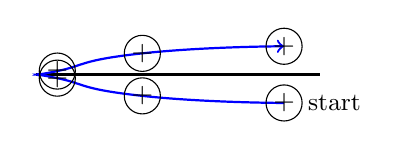
\begin{tikzpicture}[scale=0.9]
\draw[very thick] (0,0) -- (4,0);
\draw[thick, ->, blue] plot[smooth, tension=1] coordinates {(3.5,-0.4) (1.5,-0.3) (0.3,-0.05) (0.05,0.0) (0.3,0.05) (1.5,0.3) (3.5,0.4)};
\node[draw,circle,inner sep=1pt] at (3.5,-0.4) {$+$};
\node[draw,circle,inner sep=1pt] at (1.5,-0.3) {$+$};
\node[draw,circle,inner sep=1pt] at (0.3,-0.05) {$+$};
\node[draw,circle,inner sep=1pt] at (0.3,0.05) {$+$};
\node[draw,circle,inner sep=1pt] at (1.5,0.3) {$+$};
\node[draw,circle,inner sep=1pt] at (3.5,0.4) {$+$};
\node[right] at (3.7, -0.4) {\small start};
\end{tikzpicture}
\end{center}
The crosses indicate that the wheel does not rotate as it is carried around the tip --- its orientation in the lab frame is preserved.

\subsection*{(d) Reynolds number and the real-fluid flow}

The Reynolds number is the dimensionless ratio
\begin{equation}
\text{Re} = \frac{UL}{\nu},
\label{eq:Re}
\end{equation}
where $U$ and $L$ are characteristic velocity and length scales of the flow and $\nu$ the kinematic viscosity. Physically, dividing the Navier--Stokes equation $\partial_{t}\bm v + (\bm v\cdot\nabla)\bm v = -\rho^{-1}\nabla p + \nu\nabla^{2}\bm v$ through and estimating each term on dimensional grounds, the inertial term scales as $U^{2}/L$ while the viscous term scales as $\nu U/L^{2}$; their ratio is exactly $\text{Re}$. Thus $\text{Re}\gg 1$ means inertia dominates and viscosity acts only in thin boundary layers, while $\text{Re}\ll 1$ means the flow is dominated by viscous diffusion (Stokes flow).

\medskip
\noindent\emph{Two differences between potential flow and real high-Re flow about the half-plate.}

(i) \emph{Boundary layers.} A real fluid satisfies the no-slip condition $\bm v=0$ on the plate, whereas the potential solution \eqref{eq:wsqrt} permits arbitrary tangential slip. Viscosity, no matter how small, therefore generates a thin boundary layer of thickness $\delta\sim L/\sqrt{\text{Re}}$ along each side of the plate, in which the velocity is brought from its inviscid value at the edge of the layer down to zero on the plate. Vorticity of order $U/\delta$ is continuously generated at the wall and convected downstream. So a real flow has a sheath of vortical fluid clinging to the plate.

(ii) \emph{Separation and a wake; no flow round the tip.} The potential solution requires the fluid to negotiate a sharp $180^\circ$ turn at the tip, accompanied by a divergent acceleration $|\bm v|\propto r^{-1/2}$. In a real fluid the boundary layer cannot withstand the adverse pressure gradient on the upstream side of the tip and separates: instead of whipping around the tip, the flow detaches and forms a turbulent wake on the leeward side, with a region of recirculating, vortical fluid behind the plate. The shed vorticity from the boundary layers organises into a Kármán vortex street further downstream.

\medskip
\noindent\emph{Paddle-wheel motion in the real fluid.} Released at finite $r$ just below the plate, the paddle wheel is now in (or close to) the lower boundary layer, where there is real, finite vorticity $\omega \sim \partial v_{\parallel}/\partial n$ generated by the no-slip wall. The wheel therefore rotates as it is convected: it spins about its own axis as it travels along the plate. As the boundary layer separates near the tip, the wheel is shed into the wake, where it continues to rotate (and tumble irregularly in a turbulent wake) rather than executing the smooth, irrotational ride of part (c).

\begin{center}
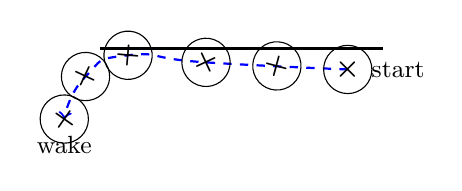
\begin{tikzpicture}[scale=0.9]
\draw[very thick] (0,0) -- (4,0);
\draw[thick, ->, blue, dashed] plot[smooth, tension=1] coordinates {(3.5,-0.3) (1.5,-0.2) (0.4,-0.1) (-0.2,-0.4) (-0.5,-1.0)};
\foreach \pt/\ang in {{(3.5,-0.3)}/0,{(2.5,-0.25)}/30,{(1.5,-0.2)}/70,{(0.4,-0.1)}/130,{(-0.2,-0.4)}/200,{(-0.5,-1.0)}/280} {
  \node[draw,circle,inner sep=2pt,rotate=\ang] at \pt {$\boldsymbol{\times}$};
}
\node[right] at (3.7,-0.3) {\small start};
\node[below] at (-0.5,-1.1) {\small wake};
\end{tikzpicture}
\end{center}
The crosses now rotate progressively, indicating that the wheel spins continuously, and the wheel ends up in the separated wake rather than reattaching to the upper side of the plate.

\medskip
\noindent\emph{Why $\text{Re}\to\infty$ does not recover potential flow.} The viscous term $\nu\nabla^{2}\bm v$ is a singular perturbation of Euler's equation: it contains the highest-order spatial derivative, so however small $\nu$ is, dropping it changes the order of the PDE and therefore the number of admissible boundary conditions. The Euler equation cannot satisfy no-slip; any real fluid with $\nu>0$ must, and does so in a boundary layer of thickness $\delta\sim L\,\text{Re}^{-1/2}\to 0$. The vorticity \emph{generated} in this thin layer is, however, $\mathcal O(U/\delta)\to\infty$; integrated against the vanishing layer thickness, the total circulation produced per unit time remains finite, and once shed into the bulk it produces $\mathcal O(1)$ wakes that persist as $\text{Re}\to\infty$. So the limit is singular: the boundary layer thins to zero, but its dynamical effect (shedding vorticity into the bulk and producing a wake) does not. This is d'Alembert's paradox in disguise: ideal-fluid theory predicts zero drag on a body in steady flow, but real flows have finite drag dominated by the wake.

\section*{Question 3 --- Internal gravity waves}

\textbf{Problem statement.} A stably stratified incompressible fluid has equilibrium density $\rho_{0}(z)$. Show that a vertically displaced parcel oscillates at the buoyancy frequency $N$. Linearise Euler about the rest state in the $x$-$z$ plane and derive the buoyancy-vorticity relation $\partial_{t}(\partial_{z}v_{x}-\partial_{x}v_{z}) = -\partial_{x}b$, with $b = -g\,\delta\rho/\rho_{0}$. Introduce a streamfunction and derive the wave equation $\partial_{t}^{2}(\nabla^{2}\psi) = -N^{2}\partial_{x}^{2}\psi$. Find the dispersion relation, prove that the group velocity is perpendicular to the phase velocity, and sketch the evolution of an internal-wave packet.

\subsection*{(a) Buoyancy frequency from a parcel argument}

Consider a fluid parcel in mechanical equilibrium at height $z_{0}$ where the surrounding fluid has density $\rho_{0}(z_{0})$. Imagine displacing the parcel quasi-statically by a small distance $\zeta$ to height $z_{0}+\zeta$. We assume:

(i) the parcel remains incompressible and exchanges no heat or mass with its surroundings, so it preserves its own density $\rho_{p} = \rho_{0}(z_{0})$;

(ii) the parcel is in pressure equilibrium with its new surroundings (the displacement is slow compared with the time for sound to traverse the parcel, so any pressure imbalance is removed acoustically); and

(iii) the displacement is small enough that we may Taylor-expand $\rho_{0}$ about $z_{0}$.

Newton's second law for the parcel, per unit volume, balances inertia against the net buoyancy force:
\begin{equation}
\rho_{p}\,\ddot\zeta = -\!\left[\rho_{p} - \rho_{0}(z_{0}+\zeta)\right]g.
\label{eq:newton-parcel}
\end{equation}
The right-hand side is just $-g$ times the density excess of the parcel over its surroundings, evaluated at the new height (a positive density excess sinks, hence the sign).

Taylor-expand $\rho_{0}(z_{0}+\zeta) \approx \rho_{0}(z_{0}) + \zeta\,\de\rho_{0}/\de z$ to first order in $\zeta$. Since $\rho_{p} = \rho_{0}(z_{0})$, equation \eqref{eq:newton-parcel} becomes
\begin{equation}
\rho_{0}(z_{0})\,\ddot\zeta = +\zeta\,g\,\frac{\de\rho_{0}}{\de z} \quad\Longrightarrow\quad \ddot\zeta + N^{2}\zeta = 0,
\label{eq:SHO}
\end{equation}
where we have defined
\begin{equation}
\boxed{\;N^{2} = -\frac{g}{\rho_{0}}\frac{\de\rho_{0}}{\de z}.\;}
\label{eq:Nsq}
\end{equation}
For a stably stratified fluid the density decreases with height ($\de\rho_{0}/\de z<0$), so $N^{2}>0$ and the parcel oscillates at the real buoyancy frequency $N$. If $N^{2}<0$ (heavier fluid above lighter fluid) the perturbation grows exponentially: this is the Rayleigh--Taylor instability.

\subsection*{(b) Linearised Euler and the buoyancy--vorticity equation}

Write the total density and pressure as the equilibrium plus a small perturbation,
\begin{equation}
\rho = \rho_{0}(z) + \delta\rho(x,z,t),\qquad p = p_{0}(z) + \delta p(x,z,t),
\label{eq:decomp}
\end{equation}
with hydrostatic balance $\de p_{0}/\de z = -\rho_{0}g$ at the equilibrium. The Euler equation for an inviscid, incompressible but variable-density fluid is
\begin{equation}
\rho\!\left(\pd{\bm v}{t} + (\bm v\cdot\nabla)\bm v\right) = -\nabla p - \rho g\hat{\bm z}.
\label{eq:eul-strat}
\end{equation}
At zeroth order the fluid is at rest. Substituting \eqref{eq:decomp} and dropping all terms quadratic in the (small) perturbation quantities $\bm v$, $\delta\rho$, $\delta p$, and using the equilibrium balance to cancel the $z$-component contribution of $p_{0}$, we obtain the linearised Euler equation
\begin{equation}
\rho_{0}\pd{\bm v}{t} = -\nabla\delta p - \delta\rho\,g\hat{\bm z}.
\label{eq:lin-euler}
\end{equation}
The $\delta\rho\,(\bm v\cdot\nabla)\bm v$ term has been dropped because it is cubic in perturbations, and the $\delta\rho\,\partial_{t}\bm v$ term as quadratic. In components,
\begin{align}
\rho_{0}\pd{v_{x}}{t} &= -\pd{\delta p}{x},\label{eq:lin-x}\\
\rho_{0}\pd{v_{z}}{t} &= -\pd{\delta p}{z} - \delta\rho\,g.\label{eq:lin-z}
\end{align}

To eliminate $\delta p$ we take $\partial_{z}$ of \eqref{eq:lin-x} minus $\partial_{x}$ of \eqref{eq:lin-z}:
\begin{equation}
\pd{}{t}\!\left(\rho_{0}\pd{v_{x}}{z} - \rho_{0}\pd{v_{z}}{x}\right) - \pd{\rho_{0}}{z}\pd{v_{z}}{t}\cdot 0\;\dots
\label{eq:cross-step}
\end{equation}
Strictly, when we differentiate $\rho_{0}\partial_{t}v_{x}$ with respect to $z$ we obtain $\rho_{0}\partial_{tz}^{2}v_{x} + (\de\rho_{0}/\de z)\partial_{t}v_{x}$. The latter is formally first-order in the small parameter $\rho_{0}^{-1}\,\de\rho_{0}/\de z$, which is $\mathcal O(N^{2}/g)$. In the standard \emph{Boussinesq approximation} for internal waves this is small compared with the other terms (one assumes that density variations are small except where they multiply $g$), and we drop it. With this approximation, after dividing through by $\rho_{0}$,
\begin{equation}
\pd{}{t}\!\left(\pd{v_{x}}{z} - \pd{v_{z}}{x}\right) = -\frac{g}{\rho_{0}}\pd{\delta\rho}{x} = -\pd{b}{x},
\label{eq:vort-buoy}
\end{equation}
where $b\equiv -g\,\delta\rho/\rho_{0}$ is the buoyancy anomaly (positive for a parcel lighter than its surroundings). Writing $\omega_{y} \equiv \partial_{z}v_{x} - \partial_{x}v_{z}$ for the (only) component of vorticity in the $x$-$z$ plane, \eqref{eq:vort-buoy} reads $\partial_{t}\omega_{y} = -\partial_{x}b$. Physically, horizontal gradients of buoyancy generate vorticity: lighter fluid to the right and heavier to the left produces an anticlockwise overturning, exactly like the sea breeze driven by differential heating.

\subsection*{(c) Streamfunction form of the wave equation}

For 2D incompressible flow, $\partial_{x}v_{x}+\partial_{z}v_{z}=0$, so we may introduce a streamfunction $\psi(x,z,t)$ with
\begin{equation}
v_{x} = \pd{\psi}{z},\qquad v_{z} = -\pd{\psi}{x}.
\label{eq:psi-def}
\end{equation}
The existence of $\psi$ is guaranteed by the Poincaré lemma applied to the closed 1-form $v_{z}\de x - v_{x}\de z$, which is closed precisely because $\partial_{x}v_{x}+\partial_{z}v_{z}=0$. With \eqref{eq:psi-def}, $\partial_{z}v_{x}-\partial_{x}v_{z} = \partial_{z}^{2}\psi+\partial_{x}^{2}\psi = \nabla^{2}\psi$, so \eqref{eq:vort-buoy} becomes
\begin{equation}
\pd{}{t}\nabla^{2}\psi = -\pd{b}{x}.
\label{eq:psi-vort}
\end{equation}

We need a second equation, namely the linearised buoyancy (or density) equation. Conservation of mass for an incompressible fluid is $\partial_{t}\rho + \bm v\cdot\nabla\rho = 0$. Linearising about $\rho_{0}(z)$,
\begin{equation}
\pd{\delta\rho}{t} + v_{z}\frac{\de\rho_{0}}{\de z} = 0 \quad\Longrightarrow\quad \pd{b}{t} = -\frac{g}{\rho_{0}}\pd{\delta\rho}{t} = \frac{g}{\rho_{0}}\frac{\de\rho_{0}}{\de z}\,v_{z} = -N^{2}\,v_{z},
\label{eq:b-eq}
\end{equation}
using $b = -g\,\delta\rho/\rho_{0}$ and the definition \eqref{eq:Nsq} of $N^{2}$. With $v_{z} = -\partial_{x}\psi$,
\begin{equation}
\pd{b}{t} = N^{2}\pd{\psi}{x}.
\label{eq:b-psi}
\end{equation}
Differentiating \eqref{eq:psi-vort} once more in time and substituting \eqref{eq:b-psi},
\begin{equation}
\pdd{}{t}\nabla^{2}\psi = -\pd{}{x}\!\pd{b}{t} = -N^{2}\pdd{\psi}{x},
\end{equation}
which is the desired internal-wave equation
\begin{equation}
\boxed{\;\pdd{}{t}\!\left(\pdd{\psi}{x}+\pdd{\psi}{z}\right) = -N^{2}\pdd{\psi}{x}.\;}
\label{eq:int-wave}
\end{equation}

\subsection*{(d) Dispersion relation, group velocity, and wave-packet sketch}

Look for plane-wave solutions of \eqref{eq:int-wave},
\begin{equation}
\psi = \mathrm{Re}\!\left[\hat\psi\,e^{i(\bm k\cdot\bm r - \omega t)}\right],\qquad \bm k = (k_{x},k_{z}).
\label{eq:plane-wave}
\end{equation}
Substituting into \eqref{eq:int-wave} we obtain $(-i\omega)^{2}(-k^{2})\hat\psi = -N^{2}(-k_{x}^{2})\hat\psi$, where $k^{2}=k_{x}^{2}+k_{z}^{2}$, i.e.\ $\omega^{2}k^{2} = N^{2}k_{x}^{2}$, giving
\begin{equation}
\boxed{\;\omega^{2} = N^{2}\,\frac{k_{x}^{2}}{k_{x}^{2}+k_{z}^{2}} = N^{2}\cos^{2}\theta,\;}
\label{eq:disp}
\end{equation}
where $\theta$ is the angle the wave vector $\bm k$ makes with the horizontal: $\cos\theta = k_{x}/k$. Strikingly, the frequency depends only on the \emph{direction} of propagation, not on the wavelength, and is bounded by $N$.

Choose without loss of generality $\omega>0$. The phase velocity is
\begin{equation}
\bm c_{p} = \frac{\omega}{k}\hat{\bm k} = \frac{N\,|\cos\theta|}{k}\hat{\bm k},
\label{eq:cp}
\end{equation}
parallel (or antiparallel) to $\bm k$. The group velocity is the gradient of $\omega$ in $\bm k$-space,
\begin{equation}
\bm c_{g} = \nabla_{\bm k}\omega = \pd{\omega}{k_{x}}\hat{\bm x} + \pd{\omega}{k_{z}}\hat{\bm z}.
\label{eq:cg}
\end{equation}
From $\omega = N k_{x}/\sqrt{k_{x}^{2}+k_{z}^{2}}$,
\begin{align}
\pd{\omega}{k_{x}} &= \frac{N}{k} - \frac{Nk_{x}^{2}}{k^{3}} = \frac{Nk_{z}^{2}}{k^{3}},\label{eq:dkx}\\
\pd{\omega}{k_{z}} &= -\frac{Nk_{x}k_{z}}{k^{3}}.\label{eq:dkz}
\end{align}
Therefore
\begin{equation}
\bm c_{g} = \frac{N k_{z}}{k^{3}}\!\left(k_{z}\hat{\bm x} - k_{x}\hat{\bm z}\right).
\label{eq:cg-explicit}
\end{equation}

Take the dot product with $\bm k$:
\begin{equation}
\bm c_{g}\cdot\bm k = \frac{N k_{z}}{k^{3}}\!\left(k_{z}k_{x} - k_{x}k_{z}\right) = 0.
\label{eq:perp}
\end{equation}
Hence $\bm c_{g}\perp\bm k$, and since $\bm c_{p}\parallel\bm k$, also $\bm c_{g}\perp\bm c_{p}$. \emph{Energy travels at right angles to the lines of constant phase} --- one of the most counter-intuitive and characteristic features of internal gravity waves.

A useful corollary: the magnitude of the group velocity is $|\bm c_{g}| = N|k_{z}|/k^{2} = N|\sin\theta|/k$. Combined with $\omega = N\cos\theta$, increasing $\theta$ (steepening the wave vector) lowers the frequency and tilts $\bm c_{g}$ towards the horizontal --- the famous ``St Andrew's cross'' pattern produced by an oscillating cylinder in a stratified fluid sees four beams emerging at the angle $\theta = \arccos(\omega/N)$ to the horizontal.

\medskip
\noindent\emph{Wave-packet evolution.} The figure shows a wave packet whose phase fronts (the dashed/streaked diagonals) make an angle $\theta$ with the horizontal $\rho_{0}=\text{const}$ surfaces, and whose wave vector $\bm k$ points up-and-to-the-right, perpendicular to the fronts. By \eqref{eq:cg-explicit}, $\bm c_{g}$ must be perpendicular to $\bm k$; the choice of sign of $\bm c_{g}$ is fixed by requiring the energy to propagate \emph{away} from the source/along $\bm c_{g}$. Taking $k_{x}>0$ and $k_{z}>0$ in the figure, $\bm c_{g}\propto (k_{z},-k_{x})$ points down-and-to-the-right.

\begin{center}
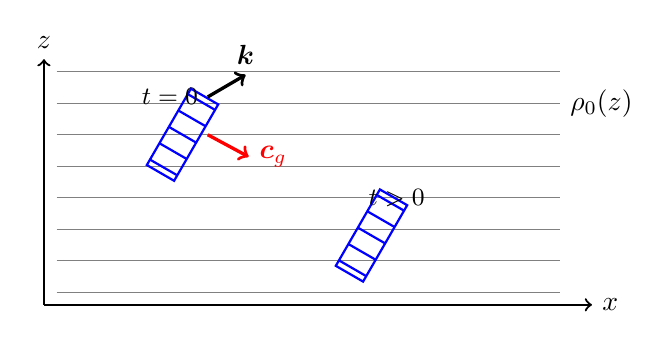
\begin{tikzpicture}[scale=0.8]
\foreach \y in {-1.5,-1,-0.5,0,0.5,1,1.5,2}{ \draw[gray] (-3,\y) -- (5,\y); }
\node[right] at (5,1.5) {$\rho_{0}(z)$};
\draw[->,thick] (-3.2,-1.7) -- (-3.2,2.2) node[above] {$z$};
\draw[->,thick] (-3.2,-1.7) -- (5.5,-1.7) node[right] {$x$};
% packet at t=0
\begin{scope}[shift={(-1,1)},rotate=60]
\draw[thick,blue] (-0.7,-0.25) rectangle (0.7,0.25);
\foreach \i in {-0.6,-0.3,0,0.3,0.6} \draw[thick,blue] (\i,-0.25) -- (\i,0.25);
\end{scope}
\node at (-1.2,1.6) {\small $t=0$};
\draw[->,very thick] (-0.6,1.6) -- (0.0,1.95) node[above]{$\bm k$};
\draw[->,very thick,red] (-0.6,1.0) -- (0.05,0.65) node[right]{$\bm c_{g}$};
% packet later
\begin{scope}[shift={(2.0,-0.6)},rotate=60]
\draw[thick,blue] (-0.7,-0.25) rectangle (0.7,0.25);
\foreach \i in {-0.6,-0.3,0,0.3,0.6} \draw[thick,blue] (\i,-0.25) -- (\i,0.25);
\end{scope}
\node at (2.4,-0.0) {\small $t>0$};
\end{tikzpicture}
\end{center}

The packet as a whole \emph{translates downward and to the right} along $\bm c_{g}$, while the individual phase fronts inside the packet move at right angles to this, namely up-and-to-the-right along $\bm k$. The phase fronts therefore appear to ``slide'' through the envelope, entering at the lower-right edge and disappearing at the upper-left edge. The packet retains its tilted shape because the dispersion relation \eqref{eq:disp} depends only on direction; all wave numbers within the packet share the same $\theta$ and hence the same group velocity.

\section*{Question 4 --- Thin-film viscous flow on an inclined plane}

\textbf{Problem statement.} A film of viscous incompressible fluid of thickness $h(x,t)$ flows under gravity down a plane inclined at angle $\theta$ to the horizontal. Write down Navier--Stokes parallel and perpendicular to the plate in the thin-film limit, state the underlying assumptions, and write down the boundary conditions. Derive the velocity profile and hence show $\partial_{t}h + \partial_{x}\!\bigl[(gh^{3}/3\nu)(\sin\theta - \cos\theta\,\partial_{x}h)\bigr] = 0$. In the limit $\theta = O(1)$, reduce to the kinematic-wave form $\partial_{t}h + u(h,\theta)\partial_{x}h \approx 0$, identify $u$, and obtain the implicit travelling-wave solution. Finally sketch the evolution of the bump shown in the figure.

\subsection*{(a) Thin-film Navier--Stokes and boundary conditions}

Set up axes with $x$ along the plate (down-slope positive) and $z$ normal to the plate, so that the plate is at $z=0$ and the free surface is at $z=h(x,t)$. The components of gravity are
\begin{equation}
\bm g = g\sin\theta\,\hat{\bm x} - g\cos\theta\,\hat{\bm z},
\label{eq:gravity}
\end{equation}
i.e.\ a down-slope component along $\hat{\bm x}$ and a normal component pressing into the plate. We make the standard \emph{lubrication} or thin-film assumptions:

(i) the film is thin, $h\ll L$, where $L$ is the typical horizontal length over which $h$ varies, so the small parameter is $\varepsilon\equiv h/L\ll 1$;

(ii) the typical velocities $u\sim U$ along the plate satisfy a low-Reynolds estimate in the appropriate sense, so the convective accelerations are small compared with viscous stresses (see below);

(iii) the flow is incompressible.

By incompressibility $\partial_{x}u+\partial_{z}w=0$, the cross-stream velocity is small, $w/u\sim\varepsilon$. The leading-order $z$-derivative is $\partial_{z}^{2}\sim 1/h^{2}$, while $\partial_{x}^{2}\sim 1/L^{2}$ is smaller by $\varepsilon^{2}$, so $\nabla^{2}u\approx\partial_{z}^{2}u$ in the thin-film limit. Likewise the convective term $u\partial_{x}u\sim U^{2}/L$ is small compared with $\nu\partial_{z}^{2}u\sim\nu U/h^{2}$ provided that the reduced Reynolds number $\varepsilon\,\text{Re}=Uh^{2}/(\nu L)\ll 1$, which we assume. Under these assumptions, the $x$- and $z$-components of Navier--Stokes reduce to
\begin{align}
0 &= -\frac{1}{\rho}\pd{p}{x} + g\sin\theta + \nu\,\pdd{u}{z},\label{eq:nsx}\\
0 &= -\frac{1}{\rho}\pd{p}{z} - g\cos\theta.\label{eq:nsz}
\end{align}
The first is the down-slope momentum balance: the pressure gradient and the parallel component of gravity drive the flow against viscous shear; in steady state on a thin film the inertia and the unsteady term are negligible. The second is hydrostatic balance in the cross-stream direction, justified because $w$ is too small for inertia or viscous stress to compete with gravity there.

The boundary conditions are:

(BC1) \emph{No-slip} on the plate, $u=0$ at $z=0$, $w=0$ at $z=0$.

(BC2) \emph{Zero shear stress} at the free surface (the air above is inviscid for our purposes): $\partial_{z}u = 0$ at $z=h(x,t)$. (More precisely, the tangential stress is continuous across the interface and the air-side stress is negligible.)

(BC3) \emph{Atmospheric pressure} at the free surface: $p = p_{\text{atm}}$ at $z=h(x,t)$. We are neglecting surface tension; otherwise BC3 would be modified by a Laplace-pressure term $-\gamma\,\partial_{x}^{2}h$.

(BC4) \emph{Kinematic condition} at the free surface: a particle on the free surface stays on it, i.e.\ $\partial_{t}h + u\,\partial_{x}h = w$ at $z=h$.

\subsection*{(b) Velocity profile and thickness equation}

Integrate \eqref{eq:nsz} from a height $z$ to the free surface $h$, using BC3 $p(h) = p_{\text{atm}}$:
\begin{equation}
p(x,z,t) = p_{\text{atm}} + \rho g\cos\theta\,[h(x,t) - z].
\label{eq:p-thinfilm}
\end{equation}
Hence
\begin{equation}
\pd{p}{x} = \rho g\cos\theta\,\pd{h}{x},
\label{eq:dpdx}
\end{equation}
which depends on $x$ but \emph{not} on $z$. The down-slope momentum equation \eqref{eq:nsx} therefore becomes
\begin{equation}
\nu\,\pdd{u}{z} = \frac{1}{\rho}\pd{p}{x} - g\sin\theta = g\!\left(\cos\theta\,\pd{h}{x} - \sin\theta\right).
\label{eq:nsx2}
\end{equation}

Integrate \eqref{eq:nsx2} once in $z$ and apply BC2 $\partial_{z}u=0$ at $z=h$ to fix the constant of integration:
\begin{equation}
\nu\,\pd{u}{z} = g\!\left(\cos\theta\,\pd{h}{x} - \sin\theta\right)(z - h).
\label{eq:dudz}
\end{equation}
Integrate again and apply no-slip $u(0)=0$:
\begin{equation}
\boxed{\;u(x,z,t) = \frac{g}{\nu}\!\left(\sin\theta - \cos\theta\,\pd{h}{x}\right)\!\left(hz - \tfrac{1}{2}z^{2}\right).\;}
\label{eq:u-profile}
\end{equation}
This is the half-Poiseuille parabolic profile: zero at the wall, maximum at the free surface, sheared by gravity (modified by the surface-slope correction).

The volumetric flux per unit width along the plate is
\begin{equation}
q(x,t) = \int_{0}^{h} u\,\de z = \frac{g}{\nu}\!\left(\sin\theta - \cos\theta\,\pd{h}{x}\right)\!\left[\tfrac{1}{2}hz^{2} - \tfrac{1}{6}z^{3}\right]_{0}^{h} = \frac{gh^{3}}{3\nu}\!\left(\sin\theta - \cos\theta\,\pd{h}{x}\right).
\label{eq:flux}
\end{equation}

Conservation of mass for an incompressible fluid in 2D, integrated through the film (using the kinematic condition BC4 to handle the moving free surface), gives the standard depth-averaged form
\begin{equation}
\pd{h}{t} + \pd{q}{x} = 0.
\label{eq:depth-mass}
\end{equation}
A direct derivation: $\partial_{t}h = w(h) - u(h)\,\partial_{x}h$ from BC4, and integrating $\partial_{x}u+\partial_{z}w=0$ from $0$ to $h$ gives $w(h) = -\partial_{x}\!\int_{0}^{h}u\,\de z + u(h)\partial_{x}h = -\partial_{x}q + u(h)\partial_{x}h$, where the boundary contribution to the Leibniz rule cancels with the kinematic condition. Subbing into BC4 yields \eqref{eq:depth-mass}. Inserting \eqref{eq:flux} we obtain the desired thickness equation,
\begin{equation}
\boxed{\;\pd{h}{t} + \pd{}{x}\!\left[\frac{gh^{3}}{3\nu}\!\left(\sin\theta - \cos\theta\,\pd{h}{x}\right)\right] = 0.\;}
\label{eq:thickness}
\end{equation}

The two terms inside the square brackets have clear physical meaning. The $\sin\theta$ term is the gravitational driving down the slope: thicker film $\Rightarrow$ heavier column $\Rightarrow$ faster flow. The $\cos\theta\,\partial_{x}h$ term is a hydrostatic-pressure correction: a positive surface slope ($\partial_{x}h>0$) gives a higher hydrostatic head upstream than downstream, opposing the gravitational drive on a slope. This is a diffusive correction that smooths sharp features in $h$.

\subsection*{(c) Kinematic-wave limit and the implicit travelling wave}

For $\theta = \mathcal O(1)$ (i.e.\ a non-shallow slope) and provided $|\partial_{x}h|\lesssim\tan\theta$, the diffusive correction in \eqref{eq:thickness} is small compared to the advective drive: $\cos\theta\,|\partial_{x}h|\ll \sin\theta$. Dropping the small term,
\begin{equation}
\pd{h}{t} + \pd{}{x}\!\left(\frac{gh^{3}\sin\theta}{3\nu}\right) = \pd{h}{t} + \frac{g\sin\theta}{3\nu}\,3h^{2}\pd{h}{x} = \pd{h}{t} + u(h,\theta)\,\pd{h}{x} = 0,
\label{eq:kw}
\end{equation}
where the kinematic-wave speed is
\begin{equation}
\boxed{\;u(h,\theta) = \frac{gh^{2}\sin\theta}{\nu}.\;}
\label{eq:kw-speed}
\end{equation}
This is exactly the surface velocity of the steady film, $u(z=h)$ from \eqref{eq:u-profile} with $\partial_{x}h$ neglected. So information about $h$ travels along the free surface at the surface velocity, three times the depth-averaged velocity $\bar u = q/h = (g\sin\theta/3\nu)h^{2}$.

Equation \eqref{eq:kw} is a first-order quasilinear PDE solved exactly by the method of characteristics. On a curve $\de x/\de t = u(h,\theta)$, we have $\de h/\de t = \partial_{t}h + u\partial_{x}h = 0$, so $h$ is constant along the characteristic. The characteristics are therefore straight lines on which $h$ takes its initial value $h_{0}(x_{0})$, and the position at later time is $x = x_{0} + u(h_{0},\theta)t$. Eliminating $x_{0} = x - u(h_{0},\theta)t$,
\begin{equation}
\boxed{\;h(x,t) \approx h_{0}\!\left(x - \frac{gh^{2}\sin\theta}{\nu}t\right),\;}
\label{eq:implicit}
\end{equation}
where $h_{0}$ is the initial profile. This is the requested implicit relation: the thickness $h$ at $(x,t)$ equals the initial thickness at the point that, moving with the wave speed $gh^{2}\sin\theta/\nu$ corresponding to that thickness, would have arrived at $(x,t)$.

\medskip
\noindent\emph{Evolution of the bump and physical interpretation.} Because the wave speed $u(h,\theta) = gh^{2}\sin\theta/\nu$ \emph{increases} with $h$, thicker parts of the film travel down-slope faster than thinner parts. The forward face of the bump (where $h$ decreases from the crest down to the foot) therefore steepens, since the higher trailing fluid catches up with the lower leading fluid. The rear face (where $h$ rises from the upstream fluid up to the crest) flattens out, since the leading higher fluid runs away from the trailing lower fluid:

\begin{center}
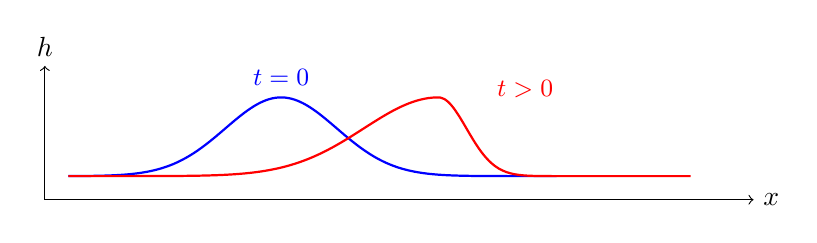
\begin{tikzpicture}[scale=1.0]
\draw[->] (-0.5,0) -- (8.5,0) node[right] {$x$};
\draw[->] (-0.5,0) -- (-0.5,1.7) node[above] {$h$};
% initial profile (smooth bump)
\draw[thick,blue,domain=-0.2:6.0,smooth,samples=80] plot (\x,{0.3 + 1.0*exp(-(\x-2.5)^2)});
\node[blue] at (2.5,1.55) {\small $t=0$};
% later: steepened front, flattened back
\draw[thick,red,domain=-0.2:7.7,smooth,samples=160] plot (\x,{0.3 + 1.0*exp(-((\x-4.5)^2)/((\x<4.5)*1.8 + (\x>=4.5)*0.25 + 0.0001 ))});
\node[red] at (5.6,1.4) {\small $t>0$};
\end{tikzpicture}
\end{center}
The forward face eventually becomes vertical: the implicit form \eqref{eq:implicit} predicts that characteristics from the bump's leading slope cross at a finite time $t^{*}$, at which point $\partial_{x}h$ becomes singular (a ``shock''). At that moment the kinematic-wave approximation ceases to be valid, because the neglected diffusive term $\cos\theta\,\partial_{x}h$ is no longer small. In a real film, the surface-slope (or surface-tension) term in \eqref{eq:thickness} regularises the shock into a finite-width travelling front. This is the same gravitational-instability phenomenon that produces fingering at the leading edge of a spreading viscous current.

\end{document}
